%=========================================================
% CAPÍTULO: Detalles de la implementación
%=========================================================

\chapter{Sistema}
\label{metodo}

En este capítulo se describen las decisiones de diseño y arquitectura del programa y los algoritmos desarrollados en este trabajo. Además se presentan de forma minimal los conceptos básicos necesarios para comprender la implementación.

El código completo se encuentra disponible en \url{https://github.com/jcevasco2003/vigs_fusion_lc}

En la Figura \ref{fig:diagrama} se muestra un diagrama que resume el proceso del sistema.

\begin{figure}[H]
    \centering
    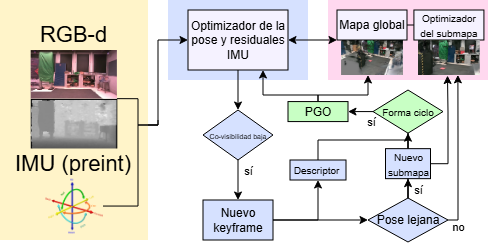
\includegraphics[width=0.9\textwidth]{../imagenes_implementacion/vigs.drawio.png}
    \caption{Los colores azul, rosa y verde representan los hilos de CPU involucrados una vez recibida la entrada de datos al sistema, enmarcada en naranja.}
    \label{fig:diagrama}
\end{figure}

%---------------------------------------------------------
% SECCIONES
%---------------------------------------------------------

\section{Heurísticas para gestión del mapa}

Como ya explicamos, la generación de gaussianas, ya sea en la inicialización o en la densificación, resulta sumamente importante para poder acelerar y corregir la optimización. Debido a que desde un punto de vista teórico no hay una forma cerrada de resolver este problema, se emplean heurísticas como la de FGS-Slam. En esta sección, presentamos otras propuestas que fueron implementadas en este trabajo como sustituto de la de Fourier, basadas en técnicas clásicas del procesamiento de imágenes. Reinterpretamos el problema de la diferenciación de frecuencias como un problema de detección de bordes, donde las regiones de alta frecuencia corresponden a bordes y texturas marcadas.

\subsection{Sobel y Laplace}

A partir del costo computacional adicional asociado a la transformada de Fourier, es natural considerar operadores locales que aproximen el contenido de alta frecuencia sin recurrir a un análisis global del espectro. En este contexto, los operadores de Sobel y Laplace resultan especialmente útiles, ya que permiten detectar cambios bruscos de intensidad de manera simple y eficiente en el dominio espacial.

\textbf{Operador de Sobel.} El operador de Sobel aproxima el gradiente de la imagen, es decir, la primera derivada espacial de la intensidad. Para una imagen $I(x,y)$, las derivadas parciales discretas en las direcciones horizontal y vertical se estiman mediante los kernels:
\begin{equation}
G_x =
\begin{bmatrix}
-1 & 0 & 1 \\
-2 & 0 & 2 \\
-1 & 0 & 1
\end{bmatrix},
\qquad
G_y =
\begin{bmatrix}
-1 & -2 & -1 \\
0 & 0 & 0 \\
1 & 2 & 1
\end{bmatrix}.
\end{equation}
La respuesta de Sobel se obtiene por convolución con la imagen:
\begin{equation}
S_x = I * G_x, \qquad S_y = I * G_y.
\end{equation}
A partir de estas componentes, la magnitud del gradiente se define como:
\begin{equation}
S = \sqrt{S_x^2 + S_y^2}.
\end{equation}
Esta magnitud resalta bordes, texturas y transiciones abruptas, por lo que constituye una aproximación local al contenido de alta frecuencia. A diferencia de Fourier, Sobel no requiere transformar la imagen al dominio frecuencial y su costo computacional es considerablemente menor, lográndose en tiempo lineal.

\textbf{Operador de Laplace.} El operador Laplace aproxima la segunda derivada espacial y, por tanto, mide la variación de la pendiente de la imagen. En dos dimensiones se define como:
\begin{equation}
\nabla^2 I = \frac{\partial^2 I}{\partial x^2} + \frac{\partial^2 I}{\partial y^2}.
\end{equation}
En versión discreta, una aproximación habitual es el kernel:
\begin{equation}
L =
\begin{bmatrix}
0 & 1 & 0 \\
1 & -4 & 1 \\
0 & 1 & 0
\end{bmatrix},
\end{equation}
o variantes equivalentes con conectividad diagonal. Su respuesta se calcula como:
\begin{equation}
L_I = I * L.
\end{equation}
La respuesta del Laplaciano enfatiza cambios rápidos de intensidad en todas las direcciones, por lo que suele destacar bordes finos y estructuras delgadas. Sin embargo, al ser una derivada de segundo orden, también es más sensible al ruido que Sobel. Aunque, del mismo modo, su complejidad temporal es lineal.

\textbf{Construcción de regiones de alta frecuencia.} En nuestra implementación, tanto Sobel como Laplace se utilizan para aproximar la distribución espacial de detalle fino. Una vez obtenida la respuesta de cada operador, se normaliza a $[0,1]$ y se aplica el mismo criterio de umbralización triangular empleado en la heurística de Fourier. Si $M_s$ y $M_l$ denotan las máscaras binarias derivadas de Sobel y Laplace, entonces las regiones de alta frecuencia quedan definidas como:
\begin{equation}
M_s(x,y)=\mathbb{I}[S(x,y)>\tau_s],
\qquad
M_l(x,y)=\mathbb{I}[L(x,y)>\tau_l],
\end{equation}
donde $\mathbb{I}[\cdot]$ es la función indicadora y $\tau_s$, $\tau_l$ son los umbrales estimados por histograma.

\subsection{Canny}

El detector de bordes de Canny constituye una alternativa más estructurada a los operadores diferenciales locales como Sobel y Laplace, ya que incorpora explícitamente un criterio de optimalidad para la detección de bordes: buena detección (baja tasa de falsos negativos), buena localización (bordes bien posicionados) y respuesta única (supresión de múltiples respuestas a un mismo borde).

A diferencia de los métodos basados únicamente en derivadas, Canny introduce un proceso en varias etapas. En primer lugar, la imagen $I(x,y)$ se suaviza mediante un filtro gaussiano para reducir el ruido:
\begin{equation}
I_\sigma(x,y) = I(x,y) * G_\sigma(x,y),
\end{equation}
donde $G_\sigma$ es un kernel gaussiano con desviación estándar $\sigma$.

Luego, se calcula el gradiente de la imagen suavizada:
\begin{equation}
G_x = I_\sigma * G_x^{Sobel}, \qquad G_y = I_\sigma * G_y^{Sobel},
\end{equation}
y su magnitud:
\begin{equation}
G = \sqrt{G_x^2 + G_y^2}.
\end{equation}

A continuación, se aplica supresión de no-máximos, que conserva únicamente los puntos que son máximos locales en la dirección del gradiente, produciendo bordes delgados (típicamente de un solo píxel). Finalmente, se aplica umbralización con histéresis, utilizando dos umbrales $\tau_{low}$ y $\tau_{high}$, definidos como:
\begin{equation}
\tau_{low} < \tau_{high}.
\end{equation}
Los píxeles con gradiente mayor a $\tau_{high}$ se consideran bordes fuertes, mientras que aquellos entre ambos umbrales se conservan únicamente si están conectados a bordes fuertes.

En la implementación utilizada en este trabajo, Canny se aplica directamente sobre la imagen en escala de grises cuantizada a 8 bits. El resultado es una máscara binaria:
\begin{equation}
M_c(x,y) =
\begin{cases}
1, & \text{si } (x,y) \in \text{bordes detectados por Canny}, \\
0, & \text{en otro caso}.
\end{cases}
\end{equation}

A diferencia de Sobel y Laplace, donde la detección de regiones de alta frecuencia depende de un umbral aplicado sobre magnitudes continuas, Canny produce directamente una segmentación binaria basada en un criterio global y contextual de bordes. Esto lo convierte en un detector más preciso y estable frente al ruido, aunque también más restrictivo en términos de densidad de activación.

En el contexto de la densificación de gaussianas, la máscara de Canny puede interpretarse como una estimación de estructura geométrica de la escena. Sin embargo, debido a su naturaleza esquelética (bordes delgados), tiende a subrepresentar regiones texturadas densas que sí son capturadas por Sobel o el análisis espectral de Fourier.


\section{Selección y muestreo de keyframes}
Un problema al tratar con optimización a tiempo real es la cantidad de datos contra el tiempo necesario para procesarlos. La cámara equipada da lugar a un flujo constante de imágenes, llamadas fotogramas o \textit{frames}, de forma tan frecuente que resulta inviable procesarlas todas. Debido a esto, se escogen de forma estratégica qué fotogramas van a ser utilizados para la optimización. Los mismos son llamados fotogramas clave, de ahora en adelante \textit{keyframes}.

La selección de keyframes es categorizada por \cite{robotics12030088} en tres tipos principales: basados en métodos probabilísticos, basados en heurísticas o basados en métodos de aprendizaje.

En el marco de este trabajo, dado un fotograma nuevo se clasifica como keyframe si cumple con un criterio de covisibilidad con el keyframe anterior menor a una cota superior. Esto quiere decir que la información que representa respecto del último keyframe es lo suficientemente nueva.

Para obtener la covisibilidad, se necesita primero calcular la visibilidad estimada de las gaussianas en ambos fotogramas por separado. En cada uno, se identifica qué gaussianas son utilizadas para renderizarlo bajo la representación actual del mundo, observando si su contribución es significativa. Luego, se utiliza una fórmula de Intersección Sobre Unión (Intersection over Union, abreviado IoE) para calcular el ratio:

Sea $G_i$ el conjunto de gaussianas que se consideran visibles,
$$
IoE (G_1, G_2) = \frac{|G_1 \cap G_2|}{|G_1 \cup G_2|} 
$$

Observemos que el denominador no debería anularse, ya que el keyframe anterior debería tener al menos una gaussiana representándolo tras los debidos pasos de optimización.



Ahora, para optimizar sobre ese conjunto de keyframes se toma una muestra que incluya el último. Esto es para no utilizar el conjunto entero, disminuyendo costos de cómputo, pero representando satisfactoriamente el espacio de interés.

Este muestreo se puede realizar de distintos modos, como utilizando distribuciones probabilísticas, tomando siempre los últimos $n$ keyframes o una combinación de ambas, muestreando n con una distribución sobre una ventana de los últimos k keyframes. 



En este trabajo, el muestreo se realizó con una distribución beta-binomial. La misma se define a partir de tres parámetros: $n$, $\alpha$ y $\beta$, y consiste en una distribución binomial de probabilidad $p$, donde $p \sim Beta(\alpha, \beta)$. De este modo, se puede interpretar como muestrear enteros $0$ a $n$ sobre una curva con forma de la distribución beta correspondiente a los parámetros. 

\begin{figure}[H]
    \centering
    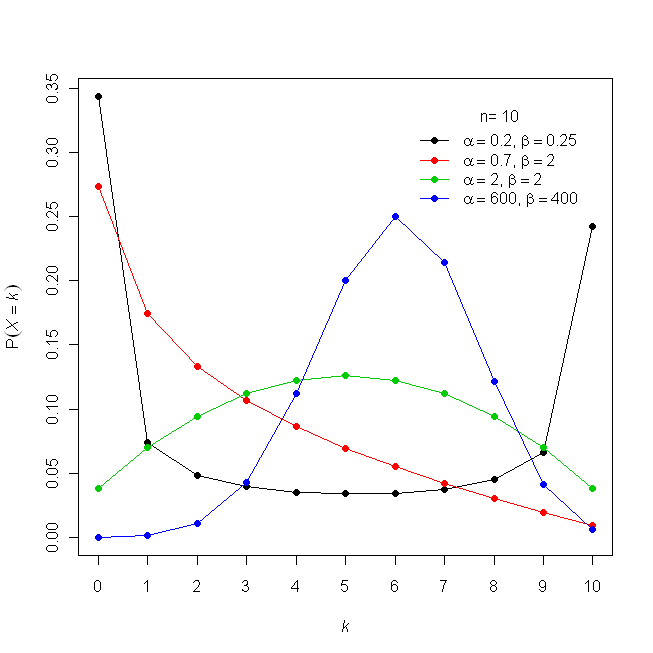
\includegraphics[width=0.8\linewidth]{../imagenes_marco_teorico/Beta-binomial_distribution.png}
    \caption{Distintas combinaciones de $\alpha$ y $\beta$ en la distribución beta binomial para n=10. Con $\alpha = 0.7$ y $\beta=2$ la distribución favorece los valores más bajos con un decaimiento hacia los más altos.}
\end{figure}

\section{Detección y cierre de ciclos}

\subsection{Submapas}

Implementamos el sistema de submapas propuesto en LoopSplat, realizando todas las operaciones que antes eran globales, como la optimización de las gaussianas en la imagen, en un marco local de cada submapa. De esta forma, cada submapa se construye a partir de un conjunto de fotogramas consecutivos, obteniendo así regiones reducidas. Si bien esto beneficia la eficiencia de las operaciones, reduce la ventaja del muestreo global de keyframes, ya que dos keyframes de submapas distintos no pueden ser comparados directamente. Esto quiere decir que la optimización pierde el mantenimiento global por sí sola. Sin embargo, en este marco el objetivo es el mantenimiento global a partir de los ciclos, enriqueciendo no solo la calidad de la representación, sino también la estimación de la pose.

\subsection{Descriptor}

Para la extracción del descriptor NetVLAD utilizamos la implementación en Python de HLoc \cite{sarlin2019coarse}, disponible en \url{https://github.com/cvg/Hierarchical-Localization} y la red preentrenada en el conjunto de datos Pitts30k, de forma análoga a LoopSplat. Esta versión de la red da lugar a descriptores de tamaño $4096$. Como nuestra implementación está escrita en C++, la integración con HLoc se realiza montando un servidor que contiene el código de extracción en Python. El cliente, es decir nuestro nodo, se comunica con el servidor entregándole la imagen a procesar y recibiendo el descriptor.

Esta implementación añade tiempos de latencia adicionales debido a los tiempos de comunicación, sin embargo, la arquitectura desacoplada de los hilos de detección de ciclos y el modelo de procesamiento por submapas permiten que esta latencia no afecte negativamente el rendimiento general del sistema. Además, facilita el acceso a posibles mejoras futuras en la red NetVLAD sin necesidad de reimplementaciones.

Es posible implementar este factor en un nodo separado de ROS2, realizando la comunicación a través de mensajes. Sin embargo, esto mantiene la latencia de comunicación, y abre la posibilidad de incompatibilidades entre las versiones de Python y dependencias entre ROS2 y HLoc. Por ello, se optó por una comunicación directa que, a su vez, permite optimizaciones en GPU.

\subsection{Heurísticas la detección de ciclos}

Para reducir el número de falsos positivos en la detección de ciclos, se implementan dos heurísticas principales. La primera es un filtro basado en la coherencia entre los centros de los submapas candidatos: si la distancia euclidiana entre los centros de las nubes de puntos de los submapas es mayor que un umbral predefinido, se descarta la correspondencia. Análogamente, si la orientación entre dos submapas no es coherente, también se descarta. La segunda heurística es el filtro por similaridad definido en el trabajo original.


\subsection{Registro de gaussianas}

En lugar de utilizar un método basado en los jacobianos de la renderización, optamos por un enfoque más clásico en SLAM basado en el registro de nubes de puntos. Para ello, reinterpretamos los centros de las gaussianas como puntos en el espacio 3D, y sus covarianzas como incertidumbres asociadas a cada punto. De esta forma, el problema de registro se convierte en un problema de alineación de nubes de puntos. Para resolverlo, empleamos una variante de ICP (\textit{Iterative Closest Point}) que tiene en cuenta las covarianzas, implementada en Open3D \cite{zhou2018open3dmodernlibrary3d}. Esta librería requiere una estimación inicial de la transformación, la cual obtenemos a partir de la pose estimada por la IMU.

\subsection{Optimización del grafo de poses}

Una vez obtenidas las correspondencias entre los submapas que cierran un ciclo, se construye un grafo de poses donde cada nodo representa la pose de un submapa y cada arista representa una restricción de transformación. Para optimizar este grafo, se utiliza la biblioteca Ceres Solver \cite{Agarwal_Ceres_Solver_2022}, que permite resolver problemas de optimización no lineal en CPU. Debido a la reducción del número de nodos como submapas, la optimización no se ve afectada significativamente por el rendimiento de la CPU.

\section{ROS2}

El programa desarrollado en este trabajo se implementó utilizando ROS2 (Sistema Operativo de Robots 2), que es una plataforma de software de código abierto ampliamente utilizada en actividades de robótica. 

ROS2 proporciona una infraestructura de comunicación entre procesos mediante un modelo de publicación y suscripción. La idea general es que los programas se organizan en nodos, que son procesos independientes que pueden comunicarse entre sí por medio de mensajes. Un nodo puede publicar mensajes en lo que se llama tópicos, que son fundamentalmente un canal de comunicación por el que transfiere un tipo de dato. Por otro lado, un nodo puede suscribirse a un tópico, lo que significa que recibirá los mensajes publicados allí. De este modo, los nodos intercambian información manteniendo la modularidad e independencia. La forma en la que se recibe un mensaje es mediante una función callback, que es una función que se ejecuta cada vez que un mensaje llega al tópico al que el nodo está suscrito.

\begin{figure}[H]
    \centering
    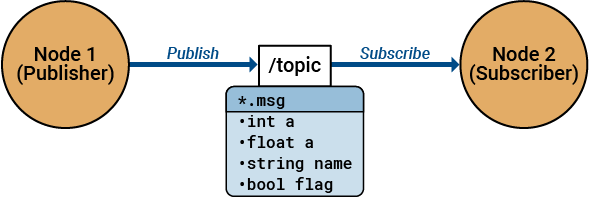
\includegraphics[width=0.8\linewidth]{../imagenes_implementacion/What-is-a-ROS2-message.png}
    \caption{Idea general de cómo funcionan los mensajes en ROS2. El nodo 1 publica mensajes en un tópico, cada mensaje con ciertos datos. El nodo 2, por su parte, se suscribe al tópico. Así, cada vez que el nodo 1 publique algún dato, el callback asociado en el nodo 2 se ejecutará. Imagen extraida de \cite{mathworks_ros2_topics}}
    \label{ros2_message}
\end{figure}

Dentro de este marco, los conjuntos de datos preparados para probar el programa funcionan como un nodo que publica los datos recopilados en los tópicos correspondientes siguiendo los tiempos originales. Es decir, funciona de forma similar a un vídeo, el cual está grabado y podemos reproducir a tiempo real cuando queramos.

Una de las limitaciones principales de ROS2 es que no posee ningún tipo de optimización para el procesamiento en GPU, esto quiere decir que el manejo de mensajes y nodos se realiza exclusivamente en CPU. De este modo, un factor limitante para la implementación es que los mensajes principales y las funciones asociadas tienen que organizarse tal que la recepción y el envío de datos resida en la memoria y en las instrucciones de la CPU.

El programa principal, contenido en un nodo, recibe como entradas los siguientes parámetros: información de la IMU, intrínsecas de las cámaras, imágenes RGB e imágenes de profundidad, estas últimas alineadas al marco de la cámara RGB. Sin embargo, no todos los conjuntos de datos cuentan con las imágenes de profundidad alineadas, por lo que, además, se implementó un nodo adicional que se encarga de registrar las imágenes, publicando así las imágenes de profundidad alineadas. Este nodo está programado en GPU, por lo que su costo es mínimo.

Como salida, el programa publica la pose estimada del robot, así como una ventana que permite visualizar el mapa reconstruido en tiempo real.







\section{Tareas en GPU}

La implementación de los filtros Sobel y Laplace es directamente paralelizable procesando cada píxel por separado. Para Fourier y Canny utilizamos librerías de NVIDIA, que ya están optimizadas para GPU.

Para el renderizado, trabajamos con una técnica estándar en este tipo de algoritmo que es el basado en tiles (o mosaicos). En esta técnica, la imagen de salida se divide en regiones de tamaño fijo, en este caso $16 \times 16$ píxeles, y cada región es procesada por un bloque de hilos en la GPU. Cada hilo dentro del bloque se encarga de calcular la contribución de las gaussianas a un píxel específico dentro de esa región. El motivo de emplear esta división es que las gaussianas contribuyen de forma significativa a un área limitada de la imagen, por lo que los píxeles de una misma región comparten muchas de las gaussianas, mientras que para regiones separadas las gaussianas relevantes varían. Así, podemos descartar muchas gaussianas según su distancia a la región, reduciendo los cálculos necesarios por píxel y aprovechando la memoria compartida del bloque para las gaussianas involucradas.

Para las jacobianas, y el resto de operaciones relacionadas, trabajamos con un hilo por gaussiana, donde el resultado numérico se acumula en la memoria global antes de ser pasado a la CPU. De este modo, y al igual que en VIGS-Fusion, la CPU solo trabaja con matrices de tamaño reducido.





\section{Hilos en CPU}

La CPU, de forma similar a la GPU, también puede ejecutar tareas en paralelo mediante el uso de hilos. Un hilo es una unidad de ejecución dentro de un proceso, y permite que diferentes partes de un programa se ejecuten simultáneamente. En este trabajo, se utilizan hilos en CPU para gestionar tareas que pueden ejecutarse con cierto grado de paralelismo pero que no requieren la potencia de una GPU ni cumplen el principio SIMD, es decir, no es posible dividirlas en partes pequeñas. Además, los hilos en CPU permiten trabajar en tareas con recursos compartidos donde los hilos se bloquean mutuamente para evitar conflictos, teniendo un sentido de orden en la ejecución.

\subsection{Hilos empleados}

Las tareas relacionadas a la localización, así como la gestión de keyframes y funciones principales, se realizan en un hilo dedicado. Esto se debe a que estas tareas requieren un orden específico y secuencial que determina el flujo de ejecución. En este hilo se encuentra la función que recibe las imágenes y la información de la IMU organizadas, encargándose tanto de la toma de decisiones (por ejemplo, si tratarla como un nuevo keyframe o no) como de la ejecución de las funciones necesarias para actualizar la pose a partir del problema de minimización. Este problema se resuelve utilizando la biblioteca Ceres, que permite resolver problemas de optimización no lineal de forma eficiente, exclusiva de CPU.

Por otro lado, un hilo distinto se encarga de optimizar el mapa, es decir, actualizar los parámetros de las gaussianas. Aquí se muestrea dentro del submapa, y luego se realiza la optimización con ADAM en GPU. De este modo, comparte con el hilo principal la información de las gaussianas, pero se bloquean cuando es necesario para evitar colisiones.

Un tercer hilo se encarga de la visualización, actualizando la ventana que muestra el mapa reconstruido en tiempo real así como las poses estimadas. Este hilo no participa en el sistema principal, sino que funciona únicamente para mostrar la información.

Del mismo modo que LoopSplat \cite{zhu2025_loopsplat}, separamos las tareas relacionadas a los ciclos en un hilo dedicado para evitar bloqueos. Así, un cuarto hilo se encarga del proceso completo de detección, verificación, registro y cierre de ciclos. Este hilo trabaja exclusivamente sobre los submapas cerrados, por lo que apenas colisiona con los hilos principales.


%=========================================================